\pdfminorversion=7
\documentclass[conference]{IEEEtran}

\usepackage[utf8]{inputenc}
\usepackage[T1]{fontenc}
\usepackage{amsmath}
\usepackage{graphicx}
\usepackage{cite}
\usepackage{booktabs}
\usepackage{float}
\usepackage{url}
\usepackage{balance}

% Keep paragraph spacing consistent without stretching the columns.
\raggedbottom

\title{Discrete Electronics Project: Class AB Audio Amplifier\\\large Design and Simulation Progress Report}

\author{
\IEEEauthorblockN{
María Fernanda Morales Calderón,
Ian José Álvarez Arrieta,\\
Óscar Felipe Montejo Cordero,
Bryan Alessandro Elizondo Fallas,
Andrés Obregón López
}
\IEEEauthorblockA{
School of Electronics Engineering\\
Tecnológico de Costa Rica (TEC)
}
}

\begin{document}
\maketitle

% Leave one line between paragraphs throughout the document body.
\setlength{\parskip}{\baselineskip}
\setlength{\parindent}{0pt}

\begin{abstract}
This paper outlines the design and simulation progress of a discrete-component Class AB audio amplifier developed in collaboration with Analog One. The system is organized into three functional sections: preamplification, amplification, and power amplification. The proposed arrangement includes an audio input network, volume adjustment, filtering, and a high-impedance preamplifier output driving subsequent stages toward an $8\,\Omega$ load. Both the preamplifier stage (using a single $+24\,\mathrm{V}$ rail) and the Class AB power stage (using $\pm24\,\mathrm{V}$ supplies) have been validated through LTspice and Multisim simulations. This report describes circuit topologies, component selections, DC operating points, time-domain transient responses using uncompressed audio streams, and AC sweep results.
\end{abstract}

\begin{IEEEkeywords}
Class AB amplifier, preamplifier, discrete electronics, BJT, MOSFET, audio amplification, LTspice, simulation.
\end{IEEEkeywords}

\section{Introduction}
An audio amplifier must increase the level of an input signal while maintaining sufficient signal quality to drive a loudspeaker. Designing an amplifier using discrete electronic components requires attention to transistor biasing, coupling networks, gain, frequency response, and the electrical conditions of the output stage. In particular, a Class AB output stage aims to reduce the high quiescent dissipation associated with Class A operation while limiting distortion around the transition between output devices.

The Discrete Electronics Project, developed in collaboration with Analog One, focuses on a Class AB audio amplifier. Its architecture is divided into three functional sections: a preamplifier, an amplifier, and a power stage. Both the preamplification stage and the power stage have been evaluated in simulation as part of the overall development process. This report summarizes the proposed organization, explains component choices across stages, and presents the analytical and simulation methods used to assess the complete amplifier system.

\section{Circuit Description}

\subsection{Preamplification Stage}
The preamplification stage processes the incoming analog audio signal—tested using the raw waveform of ``golden hour'' by JVKE—and conditions it for the subsequent gain stage. Powered from a single $V_{CC} = +24\,\mathrm{V}$ supply, the circuit employs a 2N2222A BJT in a common-emitter (CE) topology configured to drive a nominal load of $R_L = 1\,\mathrm{M}\Omega$.

Voltage-divider biasing is established by $R_{B1} = 150\,\mathrm{k}\Omega$ ($R_{10}$) and $R_{B2} = 22\,\mathrm{k}\Omega$ ($R_{11}$), maintaining $V_B \approx 3.07\,\mathrm{V}$. The collector resistor is set to $R_C = 4.3\,\mathrm{k}\Omega$ ($R_9$). To adjust the AC voltage gain so that the output signal peak remains within the $\pm1.0\,\mathrm{V_{peak}}$ range ($0\,\mathrm{dBFS}$ digital full-scale) without requiring external attenuator resistor dividers at the output, the emitter resistor $R_E$ ($R_8$) was selected as $2.2\,\mathrm{k}\Omega$. The emitter bypass capacitor ($C_E$) was deliberately omitted to provide negative feedback, stabilizing midband gain and preserving linear performance across wide dynamic ranges:
\begin{equation}
 A_v \approx \frac{R_C \parallel R_L}{R_E + r_e'} \approx \frac{4.3\,\mathrm{k}\Omega \parallel 1\,\mathrm{M}\Omega}{2.2\,\mathrm{k}\Omega + 5.6\,\Omega} \approx 1.94\,\mathrm{V/V} \quad (\approx +5.76\,\mathrm{dB}).
\end{equation}

Coupling capacitors $C_{in} = 10\,\mu\mathrm{F}$ ($C_4$) and $C_{out} = 10\,\mu\mathrm{F}$ ($C_2$) isolate DC bias levels between stages. To ensure a completely flat frequency response across the entire human audible spectrum up to $22\,\mathrm{kHz}$, the input low-pass filtering capacitor $C_1$ was set to $100\,\mathrm{pF}$ (or $1\,\mathrm{nF}$). Combined with series input resistances, the high-frequency cutoff is pushed well into the megahertz range ($f_H \approx 1.59\,\mathrm{MHz}$ for $100\,\mathrm{pF}$), guaranteeing $0.0\,\mathrm{dB}$ attenuation at $22\,\mathrm{kHz}$.

\subsection{Amplification Stage}
The amplification section provides additional voltage gain before the signal reaches the output stage. In the preliminary schematic, BS170 MOSFET common-source circuits appear within the gain path. Their bias points, gain, and interaction with the coupling capacitors must be evaluated using the corresponding transistor models.

\subsection{Class AB Power Stage}
The power stage shown in Fig.~\ref{fig:class_ab_power_stage} has already been tested in Multisim. Its role is to supply the current needed by the $8\,\Omega$ loudspeaker while following the audio signal received from the amplification stage. The $+24\,\mathrm{V}$ and $-24\,\mathrm{V}$ supplies provide room for the output signal to move in both directions around its resting level.

\begin{figure}[H]
    \centering
    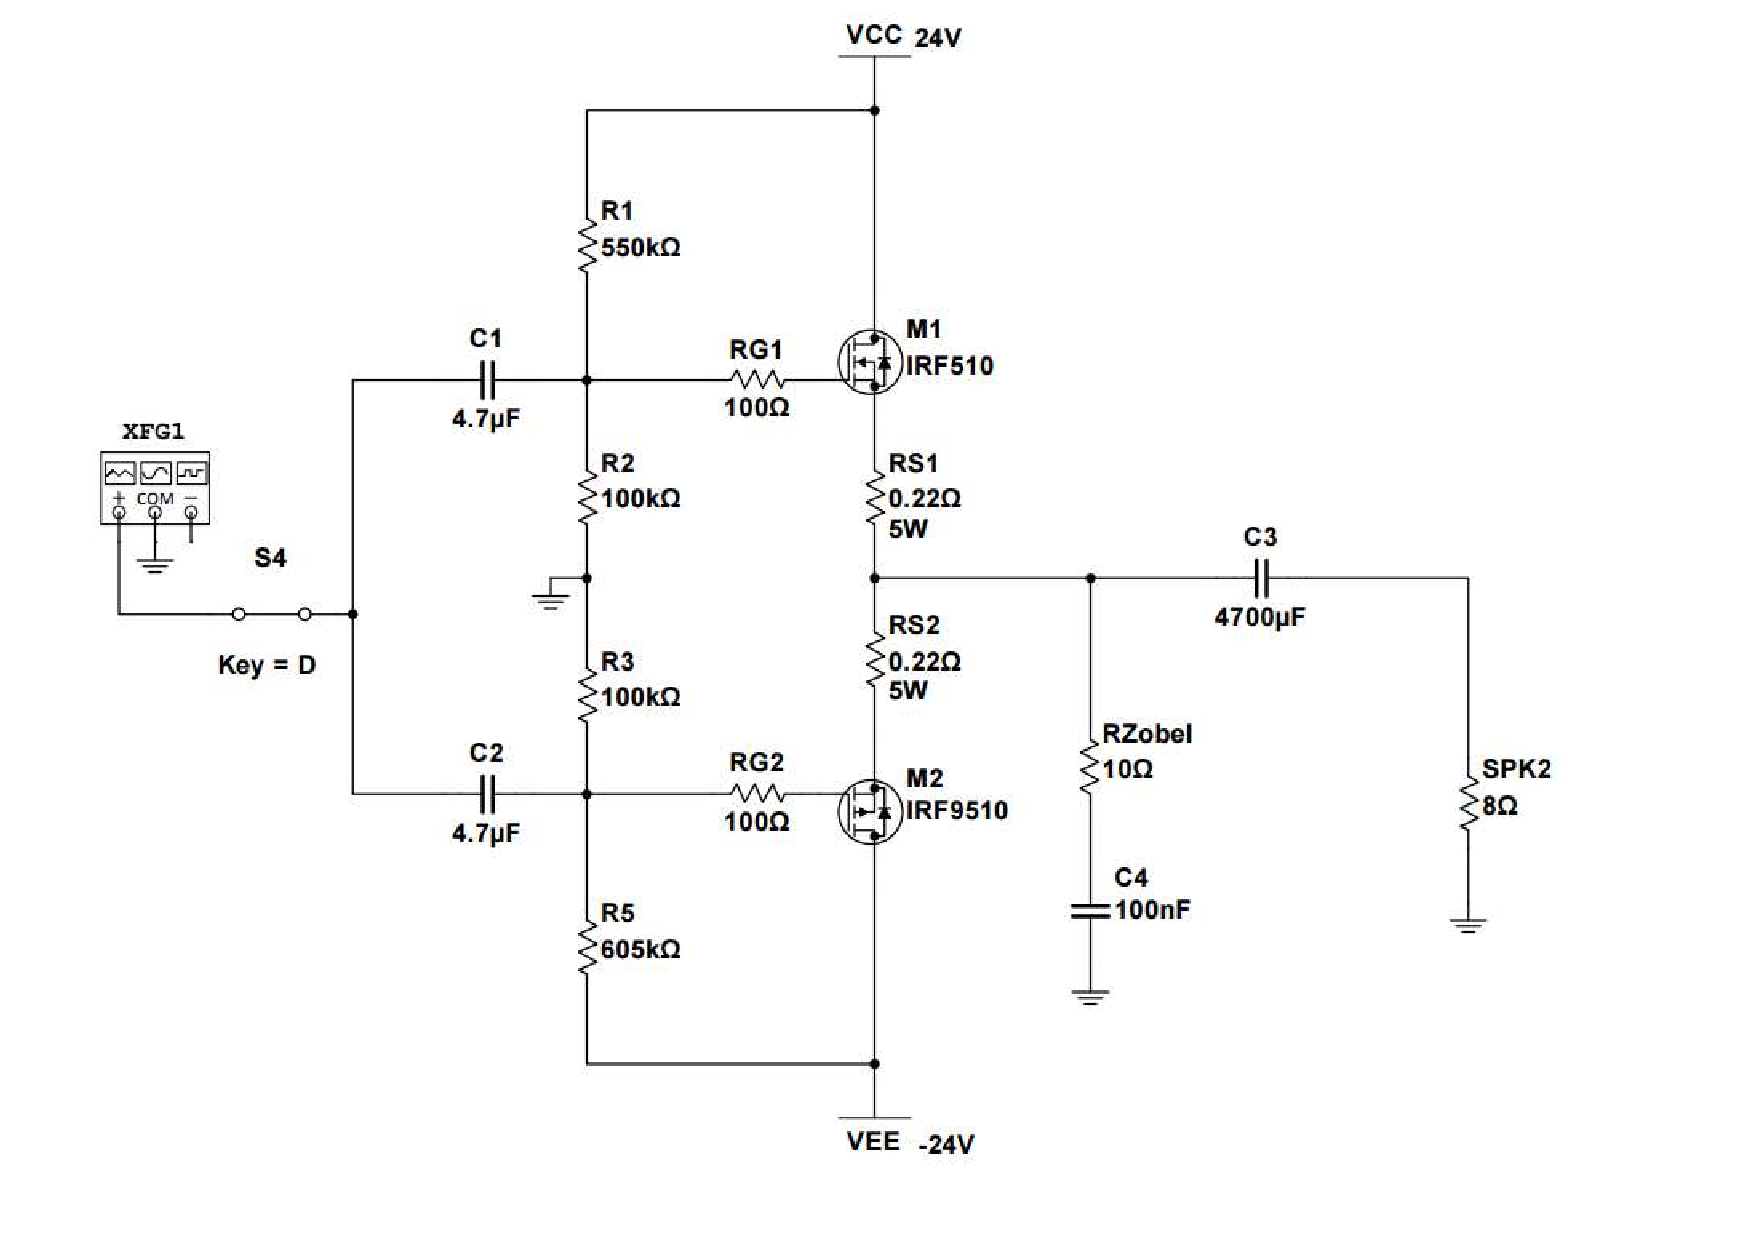
\includegraphics[width=\columnwidth]{fig/Esquematicpowersupply.pdf}
    \caption{Class AB power stage tested in simulation with an $8\,\Omega$ loudspeaker load and $\pm24\,\mathrm{V}$ supply rails.}
    \label{fig:class_ab_power_stage}
\end{figure}

The IRF510 (M1) and IRF9510 (M2) were selected as a complementary pair of power transistors. Their opposite operating polarities allow M1 to mainly handle the positive portion of the signal and M2 the negative portion. These devices provide the current-handling function required at the output, and their packages allow heat sinks to be attached for physical implementation~\cite{irf510,irf9510}.

Resistors $R_1=550\,\mathrm{k}\Omega$, $R_2=100\,\mathrm{k}\Omega$, $R_3=100\,\mathrm{k}\Omega$, and $R_5=605\,\mathrm{k}\Omega$ establish the resting conditions of the two transistors. The separate resistor ratios set their operating levels independently, while the high resistance values keep the current consumed by these networks small. Their purpose is to support a slight overlap between the activity of the devices, reducing distortion during the transition between positive and negative signal portions.

Capacitors $C_1$ and $C_2$, both $4.7\,\mu\mathrm{F}$, pass the audio signal while keeping the steady voltage of the preceding stage separate from the transistor operating levels. Together with the input resistances, their capacitance keeps attenuation of low-frequency audio small.

The $100\,\Omega$ resistors $R_{\mathrm{G1}}$ and $R_{\mathrm{G2}}$ help suppress unwanted rapid oscillations at the transistor inputs. Their role is to support stable operation while allowing the audio signal to reach both devices~\cite{mosfet_audio}.

The $0.22\,\Omega$ resistors $R_{\mathrm{S1}}$ and $R_{\mathrm{S2}}$ help stabilize the current through the output devices. Their low resistance keeps the signal voltage lost across them small. The $5\,\mathrm{W}$ rating provides capacity to dissipate the heat produced by the current flowing through these resistors.

At the output, the $4700\,\mu\mathrm{F}$ capacitor $C_3$ separates the loudspeaker from any steady voltage offset at the transistor output. This large capacitance was included because the $8\,\Omega$ load requires a substantial coupling capacitor to pass low-frequency audio with little attenuation.

The branch formed by $R_{\mathrm{Zobel}}=10\,\Omega$ and $C_4=100\,\mathrm{nF}$ helps the stage operate with a more predictable load at high frequencies. This network was included because a real loudspeaker behaves differently as frequency changes. It provides a path for high-frequency current that helps reduce unwanted oscillations, while drawing little current at lower audio frequencies~\cite{mosfet_audio}.

For the standalone simulation, XFG1 provides the test signal and S4 connects or disconnects it from the stage. In the complete amplifier, the preceding amplification stage supplies this input. The numerical results from the simulation will be presented separately from this description of the circuit and its component choices.

\section{Simulation Description}

\subsection{Simulation Environment}
Multisim and LTspice were used to simulate the audio amplifier, including the preamplification, amplification, and power stages. Both programs use mathematical models of the components to calculate voltages and currents throughout the circuit. This allows the design to be examined before physical assembly and helps identify how changes in one stage affect the others.

Multisim provides a graphical workspace with virtual instruments, such as signal generators and oscilloscopes, that support observation of the amplifier response. LTspice provides schematic-based simulation and waveform plots for examining voltages, currents, and frequency response. Both environments support the analysis of resting conditions, signal behavior over time, and operation across different frequencies.

A consistent comparison between the two simulators requires equivalent component values, supply voltages, input signals, and loudspeaker loads. The transistor models and simulation settings must also be considered when interpreting differences. For the complete amplifier, the analysis includes the connections between stages, since these connections influence the signal level and frequency response delivered to the loudspeaker.

\subsection{DC Operating-Point Analysis}
The DC operating-point analysis establishes the amplifier conditions without an applied audio signal. It calculates the steady voltages and currents that determine how the transistors are prepared to process the incoming signal. These conditions provide the starting point for interpreting the remaining simulations.

\subsubsection{Preamplifier Stage}
The DC operating-point simulation for the 2N2222A common-emitter preamplifier verified a stable Q-point under $V_{CC} = +24\,\mathrm{V}$. The base voltage set by the $R_{10}$--$R_{11}$ resistor divider yields $V_B \approx 3.07\,\mathrm{V}$, establishing an emitter voltage $V_E \approx 2.37\,\mathrm{V}$ and an emitter current $I_E \approx 1.08\,\mathrm{mA}$ across $R_8 = 2.2\,\mathrm{k}\Omega$. Collector voltage rests at $V_C \approx 19.36\,\mathrm{V}$, providing symmetric dynamic margin above ground to accommodate dynamic signal swings without saturating or clipping the transistor.

\subsubsection{Class AB Power Stage}
The DC operating-point analysis examines the resting conditions of the power stage with the $+24\,\mathrm{V}$ and $-24\,\mathrm{V}$ supplies connected. The input source is configured without a DC offset, allowing the resistor networks to establish the operating levels of M1 and M2 independently of the incoming audio signal.

The analysis focuses on the transistor voltages and the current present when no audio signal is applied. These conditions determine how the devices remain ready to reproduce the positive and negative portions of the signal and how much power is consumed while the stage is idle.

The internal output voltage is examined before capacitor $C_3$, which separates the loudspeaker from any steady voltage at this point. The resting transistor voltages and currents are obtained from the operating-point results, separately from the measurements recorded during the audio signal test.

\subsection{Transient Analysis}
Transient analysis shows how the amplifier voltages and currents change over time when an audio signal is applied. Comparing the input and output waveforms allows examination of signal amplification, changes in waveform shape, and the response of the connected stages. The input amplitude, frequency, load, and simulation interval define the conditions of each test.

\subsubsection{Preamplifier Stage}
Time-domain transient simulations (\texttt{.tran 0 10s 1s}) were executed using a direct audio file stream (\texttt{golden\_hour.wav}, $\text{AC} = 1$). Omitting the initial $1.0\,\mathrm{s}$ interval avoids transient DC coupling capacitor charging artifacts. Across the load $R_L = 1\,\mathrm{M}\Omega$ connected directly at node \texttt{out}, peak audio signal swings reach $\pm1.0\,\mathrm{V_{peak}}$, corresponding to $0.707\,\mathrm{V_{RMS}}$ peak equivalent. Due to the crest factor and dynamic range of the audio material, the integrated RMS voltage over the $9\,\mathrm{s}$ window measures approximately $290\,\mathrm{mV_{RMS}}$. Exporting the audio directly via LTspice directive \texttt{.wave "amp\_golden.wav" 16 48k V(out)} yields a clean, unclipped audio file matching standard digital full-scale limits.

\subsubsection{Class AB Power Stage}
The proposed input to the power stage is represented by a sinusoidal test signal at $10\,\mathrm{kHz}$, with a peak amplitude of $22\,\mathrm{V}$, equivalent to $44\,\mathrm{V}$ peak-to-peak. This source represents the drive signal that the preceding amplification stage is intended to provide.

With the $8\,\Omega$ load connected, the simulation recorded an output voltage of approximately $38.1\,\mathrm{V}$ peak-to-peak, equivalent to an effective value of $13.4\,\mathrm{V_{RMS}}$. The corresponding load current was approximately $1.68\,\mathrm{A_{RMS}}$, and the reported average power delivered to the load was $22.5\,\mathrm{W}$ under this test condition.

The output voltage is somewhat lower than the input voltage, consistent with the role of this stage: following the incoming signal while supplying the current required by the loudspeaker. M1 mainly handles the positive portion of the signal, while M2 mainly handles the negative portion.

The same test reported an average voltage component of approximately $1.41\,\mathrm{mV}$ across the load. This small value is consistent with capacitor $C_3$ separating the loudspeaker from the steady voltage at the transistor output.

The input and output waveforms are also examined for flattened peaks and irregularities near the transition between the two transistors. This waveform review complements the reported voltage, current, and power values when assessing signal quality.

\subsection{AC Sweep and Frequency Response}
The AC sweep examines how the amplifier responds as the input frequency changes. The resulting plots show the voltage gain and the relative phase between the input and output signals. This analysis identifies the frequency range over which the amplifier maintains a reasonably consistent response and the regions where the signal begins to decrease.

\subsubsection{Preamplifier Stage}
An AC sweep (\texttt{.ac dec 100 1 1e6}) confirmed a constant voltage gain across the entire audible spectrum ($20\,\mathrm{Hz}$ to $22\,\mathrm{kHz}$). Selecting $C_1 = 100\,\mathrm{pF}$ successfully eliminated premature high-frequency attenuation near $10\,\mathrm{kHz}$, extending the upper $-3\,\mathrm{dB}$ cutoff frequency $f_H$ past $1.0\,\mathrm{MHz}$ and maintaining $0.0\,\mathrm{dB}$ relative roll-off at $22\,\mathrm{kHz}$.

\subsubsection{Class AB Power Stage}
The frequency-response analysis examines how consistently the power stage transfers the audio signal as frequency changes. The voltage across the loudspeaker is compared with the input voltage before capacitors $C_1$ and $C_2$, allowing the response of this stage to be assessed separately from the preceding amplification stages.

The signal test at $10\,\mathrm{kHz}$ provides a reference condition, with an input of $44\,\mathrm{V}$ peak-to-peak and a recorded output of approximately $38.1\,\mathrm{V}$ peak-to-peak. These measurements describe the response during that specific signal test. The AC sweep extends the assessment across a range of frequencies using small changes around the resting operating conditions.

At low frequencies, capacitors $C_1$, $C_2$, and $C_3$ influence how much of the signal reaches the loudspeaker. At higher frequencies, the transistor characteristics, input resistors, and connections between stages influence the output level. The complete frequency-response plot is used to identify the lower and upper limits of the useful operating range.

The power-stage response is considered together with the filter and the preceding stages when assessing the audio range of the complete amplifier. The reported $22.5\,\mathrm{W}$ output belongs to the signal test at $10\,\mathrm{kHz}$; power delivery at other frequencies is assessed through the corresponding time-based tests.

\section{Results to Be Documented}
The preamplifier and power stages have been validated in simulation. Table~\ref{tab:preamp_results} records the performance parameters of the preamplifier stage, while Table~\ref{tab:power_status} outlines the current documentation status of the power stage.

\begin{table}[H]
\caption{Preamplifier Stage Simulation Results}
\label{tab:preamp_results}
\centering
\begin{tabular}{lcc}
\toprule
Parameter & Target / Value & Status \\
\midrule
Preamplifier Topology & 2N2222A CE (No $C_E$) & Validated \\
Supply Voltage ($V_{CC}$) & $+24\,\mathrm{V}$ DC & Verified \\
Midband Voltage Gain ($A_v$) & $+5.76\,\mathrm{dB}$ ($1.94\,\mathrm{V/V}$) & Verified \\
Peak Output Voltage & $\pm1.0\,\mathrm{V_{peak}}$ ($0.707\,\mathrm{V_{RMS}}$ eq.) & Verified \\
Lower Cutoff Frequency ($f_L$) & $<10\,\mathrm{Hz}$ & Verified \\
Upper Cutoff Frequency ($f_H$) & $>1.0\,\mathrm{MHz}$ ($0\,\mathrm{dB}$ at $22\,\mathrm{kHz}$) & Verified \\
Load Impedance ($R_L$) & $1\,\mathrm{M}\Omega$ & Verified \\
\bottomrule
\end{tabular}
\end{table}

\begin{table}[H]
\caption{Class AB Power Stage Documentation Status}
\label{tab:power_status}
\centering
\begin{tabular}{lc}
\toprule
Parameter & Status \\
\midrule
Power-stage simulation & Tested \\
DC bias conditions & To be documented \\
Midband voltage gain (dB) & To be documented \\
Lower cutoff frequency (Hz) & To be documented \\
Upper cutoff frequency (Hz) & To be documented \\
Output waveform and distortion & To be documented \\
Output voltage across $8\,\Omega$ & To be documented \\
\bottomrule
\end{tabular}
\end{table}

\balance

\section{Conclusions and Next Steps}
The current design organizes the Class AB audio amplifier into preamplification, amplification, and power stages. Both the preamplifier and power stage have been validated in simulation, supporting linear dynamic range expansion, current delivery, separation of steady voltages between stages, and stable signal handling. The next steps are to integrate the intermediate amplification stage, evaluate inter-stage loading effects, and prepare for physical circuit assembly. Conclusions about total gain, delivered power, distortion, bandwidth, and thermal management will be supported by integrated simulation records and physical measurements.

\begin{thebibliography}{3}

\bibitem{irf510}
Vishay Siliconix, ``IRF510: Power MOSFET,'' datasheet, document 91015, rev. D, Aug. 2021. [Online]. Available: \url{https://www.vishay.com/docs/91015/irf510.pdf}

\bibitem{irf9510}
Vishay Siliconix, ``IRF9510: Power MOSFET,'' datasheet, document 91072, rev. C, Aug. 2021. [Online]. Available: \url{https://www.vishay.com/doc?91072=}

\bibitem{mosfet_audio}
Texas Instruments, ``AN-1645 LM4702 Driving a MOSFET Output Stage,'' application report SNAA045A, May 2013, secs. 7.1--7.2. [Online]. Available: \url{https://www.ti.com/lit/an/snaa045a/snaa045a.pdf}

\end{thebibliography}

\end{document}